
%{{第三十六回}}{第三十六回}}

\chapter{绣鸳鸯梦兆绛芸轩 识分定情悟梨香院}\label{part0040_split_000.htmlux5cux23calibre_pb_0}

{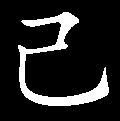
\includegraphics[width=3mm]{../Images/00003}绛芸轩梦兆是金针暗度法,夹写月钱是为袭人渐入金屋地步,梨香院是明写大家蓄戏,不免奸淫之陋。可不慎哉,慎哉!}

{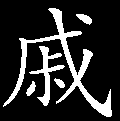
\includegraphics[width=3mm]{../Images/00005}造物何尝作主张,任人禀受福修长。划蔷亦自非容易,解得臣忠子也良。}

话说贾母自王夫人处回来,见宝玉一日好似一日,心中自是欢喜。因怕将来贾政又叫他,遂命人将贾政的亲随小厮头儿唤来,吩咐他``以后倘有会人待客诸样的事,你老爷要叫宝玉,你不用上来传话,就回他说我说了:一则打重了,得着实将养几个月才走得;二则他的星宿不利,祭了星不见外人,过了八月才许出二门。''那小厮头儿听了,领命而去。贾母又命李嬷嬷袭人等来,将此话说与宝玉,使他放心。

那宝玉本就懒与士大夫诸男人接谈,又最厌峨冠礼服贺吊往还等事,今日得了这句话,越发得了意,不但将亲戚朋友一概杜绝了,而且连家庭中晨昏定省亦发都随他的便了,日日只在园中游卧,不过每日一清早到贾母王夫人处走走就回来了,却每每甘心为诸丫鬟充役,竟也得十分闲消日月。或如宝钗辈有时见机导劝,反生起气来,只说:``好好的一个清净洁白女儿,也学的钓名沽誉,入了国贼禄鬼之流。这总是前人无故生事,立言竖辞,原为导后世的须眉浊物。不想我生不幸,亦且琼闺绣阁中亦染此风,真真有负天地钟灵毓秀之德!''{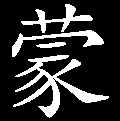
\includegraphics[width=3mm]{../Images/00006}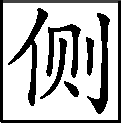
\includegraphics[width=3mm]{../Images/00011}\footnotesize \kaishu 宝玉何等心思,作者何等意见,此文何等笔墨!}因此祸延古人,除四书外,竟将别的书焚了。众人见他如此疯颠,也都不向他说这些正经话了。独有林黛玉自幼不曾劝他去立身扬名等语,所以深敬黛玉。

闲言少述。如今且说王凤姐自见金钏死后,忽见几家仆人常来孝敬他些东西,{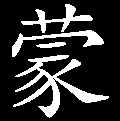
\includegraphics[width=3mm]{../Images/00006}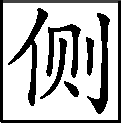
\includegraphics[width=3mm]{../Images/00011}\footnotesize \kaishu 为当涂人一笑。}又不时的来请安奉承,自己倒生了疑惑,不知何意。这日又见人来孝敬他东西,因晚间无人时笑问平儿道:``这几家人不大管我的事,为什么忽然这么和我贴近?''平儿冷笑道:``奶奶连这个都想不起来了?我猜他们的女儿都必是太太房里的丫头,如今太太房里有四个大的,一个月一两银子的分例,下剩的都是一个月几百钱。如今金钏儿死了,必定他们要弄这两银子的巧宗儿呢。''凤姐听了,笑道:``是了,是了,倒是你提醒了。我看这些人也太不知足,钱也赚够了,苦事情又侵不着,弄个丫头搪塞着身子也就罢了,又还想这个。也罢了,他们几家的钱容易也不能花到我跟前,这是他们自寻的,送什么来,我就收什么,横竖我有主意。''{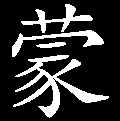
\includegraphics[width=3mm]{../Images/00006}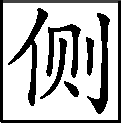
\includegraphics[width=3mm]{../Images/00011}\footnotesize \kaishu 确见高论!而其心思则不可问矣。任事者戒之!}凤姐儿安下这个心,所以自管迁延着,等那些人把东西送足了,然后乘空方回王夫人。

这日午间,薛姨妈母女两个与林黛玉等正在王夫人房里,大家吃东西呢,凤姐儿得便回王夫人道:``自从玉钏儿姐姐死了,太太跟前少着一个人。太太或看准了那个丫头好,就吩咐,下月好发放月钱的。''王夫人听了,想了一想,道:``依我说,什么是例,必定四个五个的,够使就罢了,竟可以免了罢。''凤姐笑道:``论理,太太说的也是。这原是旧例,别人屋里还有两个呢,太太倒不按例了。况且省下一两银子也有限。''王夫人听了,又想一想,道:``也罢,这个分例只管关了来,不用补人,就把这一两银子给他妹妹玉钏儿罢。他姐姐伏侍了我一场,没个好结果,剩下他妹妹跟着我,吃个双分子也不为过逾了。''凤姐答应着,回头找玉钏儿,笑道:``大喜,大喜。''玉钏儿过来磕了头。

王夫人问道:``正要问你,如今赵姨娘周姨娘的月例多少?''凤姐道:``那是定例,每人二两。赵姨娘有环兄弟的二两,共是四两,另外四串钱。''王夫人道:``可都按数给他们?''凤姐见问的奇怪,忙道:``怎么不按数给!''王夫人道:``前儿我恍惚听见有人抱怨,说短了一吊钱,是什么原故?''凤姐忙笑道:``姨娘们的丫头,月例原是人各一吊。从旧年他们外头商议的,姨娘们每位的丫头分例减半,人各五百钱,每位两个丫头,所以短了一吊钱。这也抱怨不着我,我倒乐得给他们呢,他们外头又扣着,难道我添上不成。这个事我不过是接手儿,怎么来,怎么去,由不得我作主。我倒说了两三回,仍旧添上这两分的。他们说只有这个项数,叫我也难再说了。如今我手里每月连日子都不错给他们呢。先时在外头关,那个月不打饥荒,何曾顺顺溜溜的得过一遭儿。''{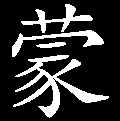
\includegraphics[width=3mm]{../Images/00006}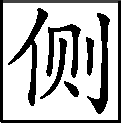
\includegraphics[width=3mm]{../Images/00011}\footnotesize \kaishu 能事能言。}王夫人听说,也就罢了,半日又问:``老太太屋里几个一两的?''凤姐道:``八个。如今只有七个,那一个是袭人。''王夫人道:``这就是了。你宝兄弟也并没有一两的丫头,袭人还算是老太太房里的人。''凤姐笑道:``袭人原是老太太的人,不过给了宝兄弟使。他这一两银子还在老太太的丫头分例上领。如今说因为袭人是宝玉的人,裁了这一两银子,断然使不得。若说再添一个人给老太太,这个还可以裁他的。若不裁他的,须得环兄弟屋里也添上一个才公道均匀了。就是晴雯麝月等七个大丫头,每月人各月钱一吊,佳蕙等八个小丫头,每月人各月钱五百,还是老太太的话,别人如何恼得气得呢。''薛姨娘笑道:``只听凤丫头的嘴,倒像倒了核桃车子的,只听他的账也清楚,理也公道。''凤姐笑道:``姑妈,难道我说错了不成?''薛姨妈笑道:``说的何尝错,只是你慢些说岂不省力。''凤姐才要笑,忙又忍住了,听王夫人示下。

王夫人想了半日,向凤姐儿道:``明儿挑一个好丫头送去老太太使,补袭人,把袭人的一分裁了。把我每月的月例二十两银子里,拿出二两银子一吊钱来给袭人。{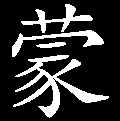
\includegraphics[width=3mm]{../Images/00006}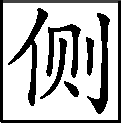
\includegraphics[width=3mm]{../Images/00011}\footnotesize \kaishu 写尽慈母苦心。}以后凡事有赵姨娘周姨娘的,也有袭人的,只是袭人的这一分都从我的分例上匀出来,不必动官中的就是了。''凤姐一一的答应了,笑推薛姨妈道:``姑妈听见了,我素日说的话如何?今儿果然应了我的话。''薛姨妈道:``早就该如此。模样儿自然不用说的,他的那一种行事大方,说话见人和气里头带着刚硬要强,这个实在难得。''王夫人含泪说道:``你们那里知道袭人那孩子的好处?{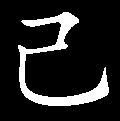
\includegraphics[width=3mm]{../Images/00003}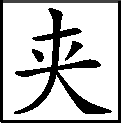
\includegraphics[width=3mm]{../Images/00012}\footnotesize \kaishu ``孩子''二字愈见亲热,故后文连呼二声``我的儿''。}比我的宝玉强十倍!{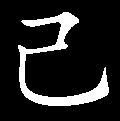
\includegraphics[width=3mm]{../Images/00003}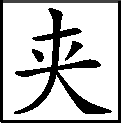
\includegraphics[width=3mm]{../Images/00012}\footnotesize \kaishu 忽加``我的宝玉''四字,愈令人堕泪,加``我的''二字者,是明显袭人是``彼的''。然彼的何如此好,我的何如此不好?又气又愧,宝玉罪有万重矣。作者有多少眼泪写此一句,观者又不知有多少眼泪也。}宝玉果然是有造化的,能够得他长长远远的伏侍他一辈子,也就罢了。''{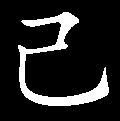
\includegraphics[width=3mm]{../Images/00003}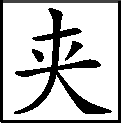
\includegraphics[width=3mm]{../Images/00012}\footnotesize \kaishu 真好文字,此批得出者。}凤姐道:``既这么样,就开了脸,明放他在屋里岂不好?''王夫人道:``那就不好了,一则都年轻,二则老爷也不许,三则那宝玉见袭人是个丫头,纵有放纵的事,倒能听他的劝,如今作了跟前人,那袭人该劝的也不敢十分劝了。{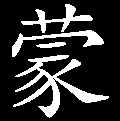
\includegraphics[width=3mm]{../Images/00006}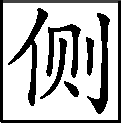
\includegraphics[width=3mm]{../Images/00011}\footnotesize \kaishu 苦心!作子弟的,读此等文章,能不坠泪?}如今且浑着,等再过二三年再说。''

说毕半日,凤姐见无话,便转身出来。刚至廊檐上,只见有几个执事的媳妇子正等他回事呢,见他出来,都笑道:``奶奶今儿回什么事,这半天?可是要热着了。''凤姐把袖子挽了几挽,跐着那角门的门槛子,{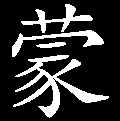
\includegraphics[width=3mm]{../Images/00006}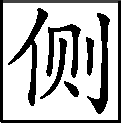
\includegraphics[width=3mm]{../Images/00011}\footnotesize \kaishu 能事得意之人,如画。}笑道:``这里过门风倒凉快,吹一吹再走。''又告诉众人道:``你们说我回了这半日的话,太太把二百年头里的事都想起来问我,难道我不说罢。''又冷笑道:``我从今以后倒要干几样尅毒事了。抱怨给太太听,我也不怕。糊涂油蒙了心,烂了舌头,不得好死的下作东西,别作娘的春梦!明儿一裹脑子扣的日子还有呢。{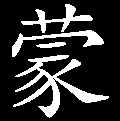
\includegraphics[width=3mm]{../Images/00006}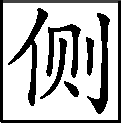
\includegraphics[width=3mm]{../Images/00011}\footnotesize \kaishu 的真活现。}如今裁了丫头的钱,就抱怨了咱们。也不想一想是奴几,也配使两三个丫头!''一面骂,一面方走了,自去挑人回贾母话去,不在话下。

却说王夫人等这里吃毕西瓜,又说了一回闲话,各自方散去。宝钗与黛玉等回至园中,宝钗因约黛玉往藕香榭去,黛玉回说立刻要洗澡,便各自散了。宝钗独自行来,顺路进了怡红院,意欲寻宝玉谈讲以解午倦。不想一入院来,鸦雀无闻,一并连两只仙鹤在芭蕉下都睡着了。宝钗便顺着游廊来至房中,只见外间床上横三竖四,都是丫头们睡觉。转过十锦槅子,来至宝玉的房内。宝玉在床上睡着了,袭人坐在身旁,手里做针线,旁边放着一柄白犀麈。宝钗走近前来,悄悄的笑道:``你也过于小心了,这个屋里那里还有苍蝇蚊子,还拿蝇帚子赶什么?''袭人不防,猛抬头见是宝钗,忙放下针线,起身悄悄笑道:``姑娘来了,我倒也不防,唬了一跳。{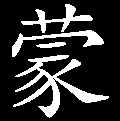
\includegraphics[width=3mm]{../Images/00006}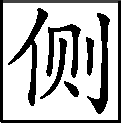
\includegraphics[width=3mm]{../Images/00011}\footnotesize \kaishu 闲情闲景,随便拈来,便是佳文佳话。}姑娘不知道,虽然没有苍蝇蚊子,谁知有一种小虫子,从这纱眼里钻进来,人也看不见,只睡着了,咬一口,就像蚂蚁夹的。''宝钗道:``怨不得。这屋子后头又近水,又都是香花儿,这屋子里头又香。这种虫子都是花心里长的,闻香就扑。''

说着,一面又瞧他手里的针线,原来是个白绫红里的兜肚,上面扎着鸳鸯戏莲的花样,红莲绿叶,五色鸳鸯。宝钗道:``嗳哟,好鲜亮活计!这是谁的,也值的费这么大工夫?''袭人向床上努嘴儿。{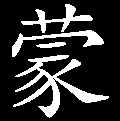
\includegraphics[width=3mm]{../Images/00006}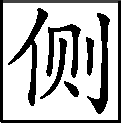
\includegraphics[width=3mm]{../Images/00011}\footnotesize \kaishu 妙形景。}宝钗笑道:``这么大了,还带这个?''袭人笑道:``他原是不带,所以特特的做的好了,叫他看见由不得不带。如今天气热,睡觉都不留神,哄他带上了,便是夜里纵盖不严些儿,也就不怕了。你说这一个就用了工夫,还没看见他身上现带的那一个呢。''宝钗笑道:``也亏你奈烦。''袭人道:``今儿做的工夫大了,脖子低的怪酸的。''{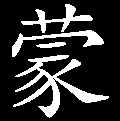
\includegraphics[width=3mm]{../Images/00006}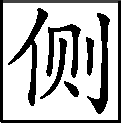
\includegraphics[width=3mm]{../Images/00011}\footnotesize \kaishu 随便写来,有神有理,生出下文多少故事。}又笑道:``好姑娘,你略坐一坐,我出去走走就来。''说着便走了。宝钗只顾看着活计,便不留心,一蹲身,刚刚的也坐在袭人方才坐的所在,因又见那活计实在可爱,不由的拿起针来,替他代刺。

不想林黛玉因遇见史湘云约他来与袭人道喜,二人来至院中,见静悄悄的,湘云便转身先到厢房里去找袭人。林黛玉却来至窗外,隔着纱窗往里一看,只见宝玉穿着银红纱衫子,随便睡着在床上,宝钗坐在身旁做针线,旁边放着蝇帚子,林黛玉见了这个景儿,连忙把身子一藏,手握着嘴不敢笑出来,招手儿叫湘云。湘云一见他这般景况,只当有什么新闻,忙也来一看,也要笑时,忽然想起宝钗素日待他厚道,便忙掩住口。知道林黛玉不让人,怕他言语之中取笑,便忙拉过他来道:``走罢。我想起袭人来,他说午间要到池子里去洗衣裳,想必去了,咱们那里找他去。''林黛玉心下明白,冷笑了两声,只得随他走了。{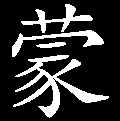
\includegraphics[width=3mm]{../Images/00006}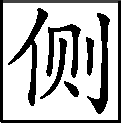
\includegraphics[width=3mm]{../Images/00011}\footnotesize \kaishu 触眼偏生碍,多心偏是痴。万魔随事起,何日是完时?}

这里宝钗只刚做了两三个花瓣,忽见宝玉在梦中喊骂说:``和尚道士的话如何信得?什么是金玉姻缘,我偏说是木石姻缘!''薛宝钗听了这话,不觉怔了。{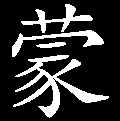
\includegraphics[width=3mm]{../Images/00006}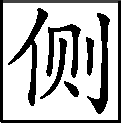
\includegraphics[width=3mm]{../Images/00011}\footnotesize \kaishu 请问:此``怔了''是呓语之故,还是呓语之意不妥之故?猜猜。}忽见袭人走过来,笑道:``还没有醒呢。''宝钗摇头。袭人又笑道:``我才碰见林姑娘史大姑娘,他们可曾进来?''宝钗道:``没见他们进来。''因向袭人笑道:``他们没告诉你什么话?''袭人笑道:``左不过是他们那些玩话,有什么正经说的。''宝钗笑道:``他们说的可不是玩话,我正要告诉你呢,你又忙忙的出去了。''

一句话未完,只见凤姐儿打发人来叫袭人。宝钗笑道:``就是为那话了。''袭人只得唤起两个丫鬟来,一同宝钗出怡红院,自往凤姐这里来。果然是告诉他这话,又叫他与王夫人叩头,且不必去见贾母,倒把袭人不好意思的。见过王夫人急忙回来,宝玉已醒了,问起原故,袭人且含糊答应,至夜间人静,袭人方告诉。{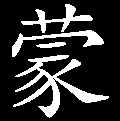
\includegraphics[width=3mm]{../Images/00006}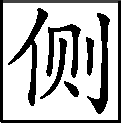
\includegraphics[width=3mm]{../Images/00011}\footnotesize \kaishu ``夜深人静''时,不减长生殿风味。何等告法?何等听法?人生不遇此等景况,实辜负此一生!}

宝玉喜不自禁,又向他笑道:``我可看你回家去不去了!那一回往家里走了一趟,回来就说你哥哥要赎你,又说在这里没着落,终久算什么,说了那么些无情无义的生分话唬我。{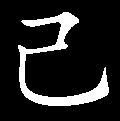
\includegraphics[width=3mm]{../Images/00003}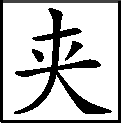
\includegraphics[width=3mm]{../Images/00012}\footnotesize \kaishu ``唬''字妙!尔果系明决男子,何得畏女子唬哉?}从今以后,我可看谁来敢叫你去。''袭人听了,便冷笑道:``你倒别这么说。从此以后我是太太的人了,我要走连你也不必告诉,只回了太太就走。''宝玉笑道:``就便算我不好,你回了太太竟去了,叫别人听见说我不好,你去了你也没意思。''袭人笑道:``有什么没意思,难道作了强盗贼,我也跟着罢。再不然,还有一个死呢。人活百岁,横竖要死,这一口气不在,听不见看不见就罢了。''{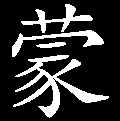
\includegraphics[width=3mm]{../Images/00006}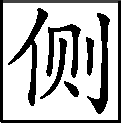
\includegraphics[width=3mm]{../Images/00011}\footnotesize \kaishu 自古及今,大凡大英雄、大豪杰,忠臣孝子,至其真极,不过一死,呜呼哀哉!}

宝玉听见这话,便忙握他的嘴,说道:``罢,罢,罢,不用说这些话了。''袭人深知宝玉性情古怪,听见奉承吉利话又厌虚而不实,听了这些尽情实话又生悲感,便悔自己说冒撞了,连忙笑着用话截开,只拣那宝玉素喜谈者问之。先问他春风秋月,再谈及粉淡脂莹,然后谈到女儿如何好,又谈到女儿死,袭人忙掩住口。

宝玉谈至浓快时,见他不说了,便笑道:``人谁不死,只要死的好。那些个须眉浊物,只知道文死谏,武死战,这二死是大丈夫死名死节。竟何如不死的好!必定有昏君他方谏,他只顾邀名,猛拚一死,将来弃君于何地!必定有刀兵他方战,猛拚一死,他只顾图汗马之名,将来弃国于何地!所以这皆非正死。''袭人道:``忠臣良将,出于不得已他才死。''宝玉道:``那武将不过仗血气之勇,疏谋少略,他自己无能,送了性命,这难道也是不得已!那文官更不可比武官了,他念两句书污在心里,若朝廷少有疵瑕,他就胡谈乱劝,只顾他邀忠烈之名,浊气一涌,即时拚死,这难道也是不得已!还要知道,那朝廷是受命于天,他不圣不仁,那天地断不把这万几重任与他了。可知那些死的都是沽名,并不知大义。{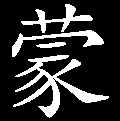
\includegraphics[width=3mm]{../Images/00006}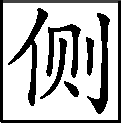
\includegraphics[width=3mm]{../Images/00011}\footnotesize \kaishu 此一段议论文武之死,真真确确,的非凡常可能道者。}比如我此时若果有造化,该死于此时的,趁你们在,我就死了,再能够你们哭我的眼泪流成大河,把我的尸首漂起来,送到那鸦雀不到的幽僻之处,随风化了,自此再不要托生为人,就是我死的得时了。''袭人忽见说出这些疯话来,忙说困了,不理他。那宝玉方合眼睡着,至次日也就丢开了。

一日,宝玉因各处游的烦腻,便想起《牡丹亭》曲来,自己看了两遍,犹不惬怀,因闻得梨香院的十二个女孩子中有小旦龄官最是唱的好,因着意出角门来找时,只见宝官玉官都在院内,见宝玉来了,都笑嘻嘻的让坐。宝玉因问:``龄官独在那里?''众人都告诉他说:``在他房里呢。''宝玉忙至他房内,只见龄官独自倒在枕上,见他进来,文风不动。{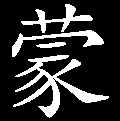
\includegraphics[width=3mm]{../Images/00006}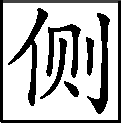
\includegraphics[width=3mm]{../Images/00011}\footnotesize \kaishu 另有风味。}宝玉素习与别的女孩子顽惯了的,只当龄官也同别人一样,因进前来身旁坐下,又陪笑央他起来唱``袅晴丝''一套。不想龄官见他坐下,忙抬身起来躲避,正色说道:``嗓子哑了。前儿娘娘传进我们去,我还没有唱呢。''宝玉见他坐正了,再一细看,原来就是那日蔷薇花下划``蔷''字那一个。又见如此景况,从来未经过这番被人弃厌,自己便讪讪的红了脸,只得出来了。宝官等不解何故,因问其所以。宝玉便说了,遂出来。{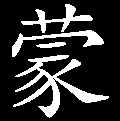
\includegraphics[width=3mm]{../Images/00006}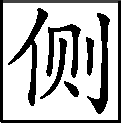
\includegraphics[width=3mm]{../Images/00011}\footnotesize \kaishu 非龄官不能如此作势,非宝玉不能如此忍{[}耐{]}。其文冷中浓,其意韵而诚,有``富贵不能移,威武不能屈''之意。}宝官便说道:``只略等一等,蔷二爷来了叫他唱,是必唱的。''宝玉听了,心下纳闷,因问:``蔷哥儿那去了?''宝官道:``才出去了,一定还是龄官要什么,他去变弄去了。''

宝玉听了,以为奇特,少站片时,果见贾蔷从外头来了,手里又提着个雀儿笼子,上面扎着个小戏台,并一个雀儿,兴兴头头的往里走着找龄官。见了宝玉,只得站住。宝玉问他:``是个什么雀儿,会衔旗串戏台?''贾蔷笑道:``是个玉顶金豆。''宝玉道:``多少钱买的?''贾蔷道:``一两八钱银子。''一面说,一面让宝玉坐,自己往龄官房里来。宝玉此刻把听曲子的心都没了,且要看他和龄官是怎样。只见贾蔷进去笑道:``你起来,瞧这个顽意儿。''龄官起身问是什么,贾蔷道:``买了雀儿你顽,省得天天闷闷的无个开心。我先顽个你看。''说着,便拿些谷子哄的那个雀儿在戏台上乱串,衔鬼脸旗帜。众女孩子都笑道``有趣'',独龄官冷笑了两声,赌气仍睡去了。贾蔷还只管陪笑,问他好不好。龄官道:``你们家把好好的人弄了来,关在这牢坑里学这个劳什子还不算,你这会子又弄个雀儿来,也偏生干这个。你分明是弄了他来打趣形容我们,还问我好不好。''贾蔷听了,不觉慌起来,连忙赌身立誓。又道:``今儿我那里的香脂油蒙了心!费一二两银子买他来,原说解闷,就没有想到这上头。罢,罢,放了生,免免你的灾病。''{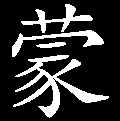
\includegraphics[width=3mm]{../Images/00006}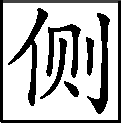
\includegraphics[width=3mm]{../Images/00011}\footnotesize \kaishu 此一番文章从``划蔷''而来,``蔷''之划为不谬矣。}说着,果然将雀儿放了,一顿把将笼子拆了。龄官还说:``那雀儿虽不如人,他也有个老雀儿在窝里,你拿了他来弄这个劳什子也忍得!今儿我咳嗽出两口血来,太太叫大夫来瞧,不说替我细问问,你且弄这个来取笑。偏生我这没人管没人理的,又偏病。''说着又哭起来。贾蔷忙道:``昨儿晚上我问了大夫,他说不相干。他说吃两剂药,后儿再瞧。谁知今儿又吐了。这会子请他去。''说着,便要请去。龄官又叫``站住,这会子大毒日头地下,你赌气子去请了来我也不瞧。''贾蔷听如此说,只得又站住。宝玉见了这般景况,不觉痴了,这才领会了划``蔷''深意。{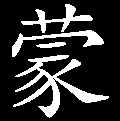
\includegraphics[width=3mm]{../Images/00006}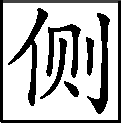
\includegraphics[width=3mm]{../Images/00011}\footnotesize \kaishu 点明。}自己站不住,也抽身走了。贾蔷一心都在龄官身上,也不顾送,倒是别的女孩子送了出来。

那宝玉一心裁夺盘算,痴痴的回至怡红院中,正值林黛玉和袭人坐着说话儿呢。宝玉一进来,就和袭人长叹,说道:``我昨晚上的话竟说错了,怪道老爷说我是`管窥蠡测'。昨夜说你们的眼泪单葬我,这就错了。我竟不能全得了。从此后只是各人各得眼泪罢了。''{\includegraphics[width=3mm]{../Images/00006}\includegraphics[width=3mm]{../Images/00011}\footnotesize \kaishu 这样悟了,才是真悟。}袭人昨夜不过是些顽话,已经忘了,不想宝玉今又提起来,便笑道:``你可真真有些疯了。''宝玉默默不对,自此深悟人生情缘,各有分定,只是每每暗伤``不知将来葬我洒泪者为谁?''此皆宝玉心中所怀,也不可十分妄拟。

且说林黛玉当下见了宝玉如此形像,便知是又从那里着了魔来,也不便多问,因向他说道:``我才在舅母跟前听的明儿是薛姨妈的生日,叫我顺便来问你出去不出去。你打发人前头说一声去。''宝玉道:``上回连大老爷的生日我也没去,这会子我又去,倘或碰见了人呢?我一概都不去。这么怪热的,又穿衣裳,我不去姨妈也未必恼。''袭人忙道:``这是什么话?他比不得大老爷。这里又住的近,又是亲戚,你不去岂不叫他思量。你怕热,只清早起到那里磕个头,吃钟茶再来,岂不好看。''宝玉未说话,黛玉便先笑道:``你看着人家赶蚊子分上,也该去走走。''宝玉不解,忙问:``怎么赶蚊子?''袭人便将昨日睡觉无人作伴,宝姑娘坐了一坐的话说了出来。宝玉听了,忙说:``不该。我怎么睡着了,亵渎了他。''一面又说:``明日必去。''

正说着,忽见史湘云穿的齐齐整整的走来辞,说家里打发人来接他。宝玉林黛玉听说,忙站起来让坐。史湘云也不坐,宝、林两个只得送他至前面。那史湘云只是眼泪汪汪的,见有他家人在跟前,又不敢十分委曲。少时薛宝钗赶来,愈觉缱绻难舍。还是宝钗心内明白,他家人若回去告诉了他婶娘,待他家去又恐受气,因此倒催他走了。众人送至二门前,宝玉还要往外送,{\includegraphics[width=3mm]{../Images/00003}\includegraphics[width=3mm]{../Images/00012}\footnotesize \kaishu 每逢此时就忘却严父,可知前云``为你们死也情愿''不假。}倒是湘云拦住了。一时,回身又叫宝玉到跟前,悄悄的嘱道:``便是老太太想不起我来,你时常提着打发人接我去。''宝玉连连答应了。眼看着他上车去了,大家方才进来。要知端的,且听下回分解。

{\includegraphics[width=3mm]{../Images/00005}总评:绛芸轩梦兆是金针暗渡法,夹写月钱是为袭人渐入金屋地步,梨香院是明写大家蓄戏,不免奸淫之陋。可慎哉,慎哉!}
